\chapter{L'arborescence}

L'arborescence sous Linux correspond à la manière sont agencés les dossiers (directory en anglais) les uns par rapport aux autres.

\begin{center}
	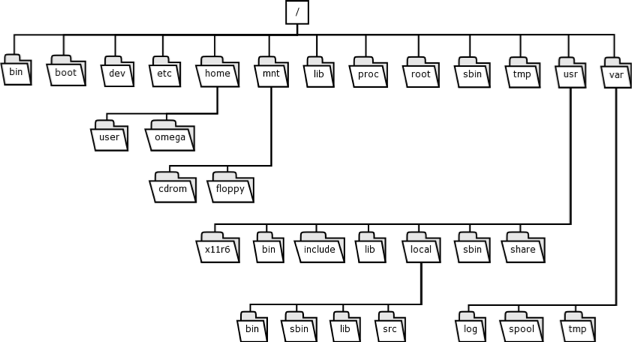
\includegraphics[width=0.7\textwidth]{Images/arborescence.png}
	\captionof{figure}{Arborescence d'un système GNU/Linux}
\end{center}

Vous l'aurez peut être remarqué mais tous les dossiers mènent à /. Ce dossier a pour petit nom, root. Il est ce que l'on appelle la racine du système. De ce dossier découle une floppé d'autre. Chacun à son utilité, nous allons voir quelques uns ensemble.
\begin{itemize}
	\item home : ce dossier contient les fichiers des utilisateurs. C'est ici que se situe les données des utilisateurs.
	\item usr : ce dossier contient tous les binaires de l'utilisateur, leur documentation, des librairies, des header, etc …
	\item mnt : ce dossier est le dossier conventionnel pour monter des volumes (clé usb, lecteur cd, etc …). Il est possible de monter un volume où l'on veut dans son arborescence mais le système va monter par defaut les volume dans ce dossier.
	\item var : dans ce dossier se situe les applications/programmes installé par l'utilisateur.
\end{itemize}
